 %%%%%%%%%%%%%%%%%%%%%%%%%%%%%%%%%%%%%%%%%% 
 % @File    : c:\Users\Administrator\Desktop\GNN\tutorial\sections\GCN-math.tex
 % @Date    : 2020-12-08 17:19:56
 % @Author  : RankFan
 % @Email   : 1917703489@qq.com
 % -----
 % Last Modified: 2020-12-09 15:11:38
 % Modified By: Rank_fan
 % -----
 %%%%%%%%%%%%%%%%%%%%%%%%%%%%%%%%%%%%%%%%%% 

\section{GNN-Math}
     \subsection{Laplace Operator}
     如果 $ f $ 是欧式空间中的二阶可微实函数,那么 $ \Delta \cdot $ (divergence)为拉普拉斯算子, 物理上,散度的意义是场的有源性。 $ \Delta f $ 就是在欧式空间中求其二阶微分({\textbf{散度}})。
     $ div(F)>0 $ 表示该点有散发通量的正源(发散源);$ div(F)= 0 $ 表示该点无源;$ div(F)< 0 $ 表示该点有吸收能量的负源(洞或汇)。
     
     $ \nabla ^{2}f $ 又可以写成  $ \nabla  \cdot \nabla  f $。梯度 “$ \nabla $ ”的本意是一个向量,表示某一个函数在该点处的方向导数沿着该方向取得最大值,即函数的在该方向沿着此方向的梯度方向上升或下降最快



     图的拉普拉斯矩阵,如果把它看作一个线性变换,它起的作用是和数学分析中的拉普拉斯算子是一样的,即拉普拉斯矩阵就是图上的拉普拉斯算子,或者说是离散的拉普拉斯算子。

     如果$ f $ 是图上定义的一组高维向量(特征),那么$ L f $就是在图空间求其二阶微分(散度),$ L $ 是图的拉普拉斯矩阵。

     \begin{myExample}
        $ u = f(x,y) $ 在空间区域 $ G $ 是一阶连续可导($ C ^{1}$) ,点 $ P(x,y) \in G $ 处的梯度向量为:
        \[ \left \{ \frac{\partial f}{\partial x} , \frac{\partial f}{\partial y} 
        \right \}  = \frac{\partial f}{\partial x} \overrightarrow{i} + \frac{\partial f}{\partial y} \overrightarrow{j} \]
        记为$grad \, f(x,y)$ 或 $ \nabla f(x,y)$ 。其中:$ \nabla = \frac{\partial }{\partial x} \overrightarrow{i} + \frac{\partial }{\partial y} \overrightarrow{j}$
        称为(二维)向量的微分算子或 Nabla 算子。
     \end{myExample}

     拉普拉斯算子(Laplace Operator)是 $ n $ 维欧几里得空间中的一个二阶微分算子,定义梯度($ \nabla $ )的散度为 $ \Delta \cdot $ 

     \begin{equation}
        \nabla ^{2}f = \nabla  \cdot \nabla  f  = div(grad \, f )
     \end{equation}

     \begin{myExample}[离散形式的拉普拉斯算子]
        下面以二维为例,每个维度的变化最小单位为1,
        \begin{align*}
            \frac{\partial f}{\partial x} & = f^{\prime} (x) = f(x+1) - f(x) \\
            \frac{\partial^{2} f}{\partial x^{2}} &  =   f^{\prime \prime } (x)   \approx f^{\prime }(x) - f^{\prime }(x-1) 
             = f(x+1) + f(x-1) -2f(x) \\
            \Longrightarrow \Delta f & =   \frac{\partial^{2} f}{\partial x^{2}} +\frac{\partial^{2} f}{\partial y^{2}} \\ 
            & = f(x+1,y) + f(x-1,y) + f(x,y+1) + f(x,y-1) -4f(x,y)  
        \end{align*}
     \end{myExample}
     
     \begin{myRemark}
        如果$ \Delta f = 0 $,可以近似认为中心点 $ f(x,y) $ 的势和其周围点的势是相等的, $ f(x,y) $ 局部范围内不存在势差,所以该点无源。
        如果$ \Delta f > 0 $,可以近似认为中心点 $ f(x,y) $ 的势低于周围点,可以想象成中心点如恒星(太阳)一样发出能量,补给周围的点,所以该点是正源。
        如果$ \Delta f < 0 $,可以近似认为中心点 $ f(x,y) $ 的势高于周围点,可以想象成中心点如吸引子一样在吸收能量,所以该点是负源。
     \end{myRemark}

     另一个角度,拉普拉斯算子计算了周围点与中心点的梯度差。当 $ f(x,y) $  受到扰动之后,其可能变为相邻的$ f(x+1,y) , f(x-1,y) , f(x,y+1) , f(x,y-1)  $之一,拉普拉斯算子得到的是对该点进行微小扰动后可能获得的总\href{https://www.zhihu.com/question/22104055/answer/1236811448}{增益}(或者说是总变化)。

     将这个结论推广到图,假设具有$ N $个节点的图$ G $,此时以上定义的函数f将是$ N $维向量:$ f = (f_1,f_2,f_3,...,f_N) $。其中$ f_i $ 为函数f在图中节点$ i $处函数的值,类比于$ f(x,y) $在节点
     (x,y)处的值。对$ i $ 节点进行扰动,它可能变为任意一个与它相邻的节点 $ j \in N_i $, $ N_i $ 表示节点i的一阶领域点。
     \begin{figure}[htb!]
        \centering
        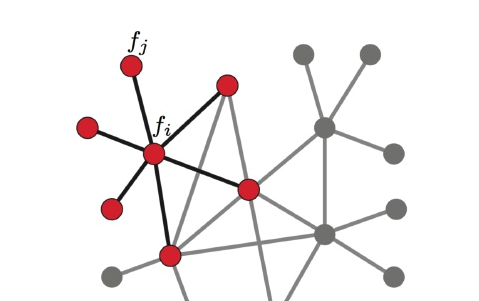
\includegraphics[scale = 0.7 ] {node_graph.png}
        \caption{图结构}
     \end{figure}

     我们上面已经知道拉普拉斯算子可以计算一个点到它所有自由度上微小扰动的增益,则通过图来表示就是任意一个节点 $ j $ 变化到节点$ i $ ,假设图中边的权值相等(简单说就是1 , $ w_{ij} = 1 $)则

     \begin{align*}
         \Delta f_{i} = \sum_{j \in N_{i}} (f_i - f_j) = \sum_{j \in N_{i}} \left [ w_{ij} (f_i - f_j) \right ] 
     \end{align*}

     由于当  $ j \notin  N_{i} \Longrightarrow w_{ij} = 0 $,此时$ i,j $不相邻。
     \begin{align*}
         \sum_{j \in N }  \left [ w_{ij} (f_i - f_j) \right ] &  = \sum_{j \in N } w_{ij}f_i - \sum_{j \in N } w_{ij} f_j \quad d_i \triangleq  \sum_{j \in N } w_{ij}   \\
           & = d_{i} f_{i} -w_{i:}f
    \end{align*}

    $ w_{i:} = (w_{i,1},w_{i,2},\dots,w_{i,N} )$  是$ N $维行向量,$ f = (f_{1},f_{2},\dots,f_{N} )$ 。$ w_{i:}f $ 表示两个向量之间的内积。$ D_{n \times n} $度矩阵,$ W_{n \times n} $ 为邻接矩阵。    $L = D-W $

    \begin{myRemark}
        拉普拉斯矩阵中的第 $ i $ 行实际上反应了第 $ i $ 个节点在对其他所有节点产生扰动时所产生的增益累积。直观上来讲,图拉普拉斯反映了当我们在节点$ i $ 上施加一个势,
        这个势以哪个方向能够多顺畅的流向其他节点(梯度的感觉)。谱聚类中的拉普拉斯矩阵可以理解为是对图的一种矩阵表示形式。
    \end{myRemark}

    \begin{align*}
        \Delta f & =    \left(\begin{array}{c}
            \Delta f_{1} \\
            \vdots \\
            \Delta f_{N}
            \end{array}\right)=\left(\begin{array}{c}
            d_{1} f_{1}-w_{1:} f \\
            \vdots \\
            d_{N} f_{N}-w_{N:} f
            \end{array}\right)  \\
            & =  \left(\begin{array}{ccc}
                d_{1} & \cdots & 0 \\
                \vdots & \ddots & \vdots \\
                0 & \cdots & d_{N}
                \end{array}\right) f-\left(\begin{array}{c}
                w_{1:} \\
                \vdots \\
                w_{N:}
                \end{array}\right) f \\
            & =\operatorname{diag}\left(d_{i}\right) f-W f \\
            & ={\color{myred} (D-W)}f \\
            &={\color{myred} L } f
    \end{align*}


  \subsection{GCN-Spectral Based}       

 
    特征函数与傅里叶算子:
    \begin{align}
        F(w) = \mathcal{F}\left [ f(t) \right ] = \int_{ t } f(t)e^{-iwt}\mathrm{ dt } \\
        e^{-iwt} = cos(wt) - isin(wt) 
    \end{align}
 
    开始我的表演:
    首先 $ \hat{x} = A \boldsymbol x $表示的含义是对x所在的空间进行了转换,如果A的列向量是$ n $个基向量,表示x转换到A的 $ n $个基向量所表征的空间内, $ A \boldsymbol x  = \lambda \boldsymbol x $ ,$ \lambda $是一个scale,这里表示的空间转换仅仅是在
     $ \boldsymbol x $ 进行一个放缩,也就是这个向量($ \boldsymbol x $)是$ A $一个特征向量。
    如果特征向量是基向量,这就意味着进行空间转换也就是对坐标轴进行放缩。

    \begin{align}
        \Delta e^{-iwt} = \frac{\partial^2 e^{-iwt}}{\partial t^2} = \frac{\partial -iwe^{-iwt}}{\partial t} = i^{2} w^{2}e^{-iwt} = -w^{2}e^{-iwt} 
    \end{align}
    
    \[
        \Delta  \tikzmark{identity}{\texttt{ $ e^{-iwt} $ }} = -\tikzmark[red]{G}{ \texttt{$ w^{2} $} }
    \tikzmark[blue]{L}{\texttt{$ e^{-iwt} $}}
    \]
        %  \Delta   \tikzmark{identity}{\texttt{I}}= ( -\tikzmark[red]{G}{ \texttt{G} }
        % \tikzmark[blue]{L}{ \texttt{L} )
  
        % (\tikzmark{identity}{$ \Delta $} \tikzmark[red]{G}{\texttt{G})  = ( -\tikzmark[red]{G}{\texttt{$ w^{2}$}}
        % \tikzmark[blue]{L}{\texttt{$ e^{-iwt} $}} )
    \begin{tikzpicture}[overlay, remember picture,node distance =1.5cm]
        \node (identitydescr) [below left = of identity ]{Eigenvalue};
        \draw[,->,thick] (identitydescr) to [in=-90,out=90] (identity);
        \node[red] (Gdescr) [below right = of G]{Frequency};
        \draw[red,->,thick] (Gdescr) to [in=-90,out=90] (G);
    \end{tikzpicture}

    \begin{align}
        \hat{f} & = u^{T}x \Longrightarrow \hat{y} = {\color{myred} g_{\theta} \star x} = g_{\theta} (\Lambda) \hat{x} =  g_{\theta} (\Lambda) u^{T}x   \Longrightarrow \\
        y  & = \left( u^{T}\right) ^{-1} \hat{y} =  u g_{\theta} (\Lambda)  \hat{x} = g_{\theta} ({\color{myred}u \Lambda u^{T}}) x = g_{\theta} ({\color{myred}L}) x \\
        L_{reg} & =  \sum_{i} \sum_{j} W_{ij}  \left \| f(X_{i}) -f(X_{j}) \right \|  =f ^{T} (X) L f(X) \\
        L & = I_{n} - D^{-\frac{1}{2}}W D^{-\frac{1}{2}} = u \Lambda u^{T}
    \end{align}

    \begin{myRemark}
        $ L _{n \times n}$ 在无向图中是一个实对称阵,实对称阵可对正交对角化,n个不同的特征向量可以表示n个基向量(Independent)。$ u ^ { T } _{ n \times n }f _{n \times 1 }$表示将f所在的空域转换为时域,$g_{\theta} $ 表示一个关于$ \theta $的 $ n \times n $的对角矩阵,其中的参数也就是机器学习要学习的参数。$ \Lambda _{ n \times n }$ 为 L的正交对角化矩阵,$ u u ^ { T }  = I $。

        \[
            \hat{x} =  \begin{pmatrix}
                \hat{f}\left ( {\lambda 1} \right )  \\
                \hat{f}\left ( {\lambda 2} \right )  \\
                \vdots\\
                \hat{f}\left ( {\lambda n} \right )  \\
                
                \end{pmatrix} 
            = \begin{pmatrix}
                u_{1} \left ( 1 \right ) &  u_{1} \left ( 1 \right ) & \cdots&  u_{1} \left ( n \right )& \\
                u_{2} \left ( 1 \right ) &  u_{2} \left ( 2 \right ) & \cdots&  u_{2} \left ( n \right )&\\
               \vdots & \vdots & \vdots &  \vdots& \\
                 u_{n} \left ( 1 \right ) &  u_{n} \left ( 2 \right ) & \cdots&  u_{n} \left ( n \right )&
              \end{pmatrix} 
              \begin{pmatrix}
                f\left ( { 1 } \right )  \\
                f\left ( { 2 } \right ) \\
                \vdots\\
                f\left ( { n } \right )  \\
             \end{pmatrix}\]
        \begin{align*} 
            \hat{f} \left ( {\lambda 1} \right )   & =  u_{1} \left ( 1 \right ) f(1) + u_{1} \left ( 2 \right ) f(2) + \cdots + u_{1} \left ( n \right ) f(n) = \sum_{i = 1} ^{n}  u_{1} \left ( i \right ) x(i) \Longrightarrow \\
            \hat{f\left ( {\lambda_{\ell }} \right )}  & = \sum_{i = 1} ^{n}  u_{\ell } \left ( i \right ) f(i)   = \int u_{\ell } \left ( i \right ) f(i) \mathrm{d i}  \quad \ell  = 1 , 2 ,\dots , n  
        \end{align*}
    \end{myRemark}
    \begin{myExample}[傅里叶逆变换]
    \begin{align*}
        f(t) & = \mathcal{F}^{-1} \left( F(w) \right) = \frac{1}{2\pi} \int F(w) e^{iwt} \mathrm{dw}  \\
        f * h  & = \mathcal{F}^{-1} \left( \hat{f(w)} * \hat{h(w)}  \right) = \frac{1}{2\pi} \int \left( \hat{f(w)} * \hat{h(w)}  \right)  \mathrm{dw} \\
        ( f * h ) _{G}  & = u \, diag\left [  \hat{h(w)} \right ] u^{T} f  =u \, diag\left [   u^{T} h  \right ] u^{T} f  = u \left[  (u^{T} h) \odot (u^{T} f)  \right]
    \end{align*} 
    
        \begin{myRemark}
            $ \odot $ 表示Hadamard product(哈达马积),对于两个维度相同的向量、矩阵、张量进行对应位置的逐元素乘积运算。$ h $ 为卷积核 ,$\hat{h}$ 为 $h$ 的傅里叶变化,这里的 $diag\left [  \hat{h(w)} \right ] $ 是上文中所说的 $g_{\theta} (\Lambda)$ 的另一种形式, $\lambda$ 在频域中和频率表示一个含义。
        \end{myRemark}
        \[
            diag(\hat{h}) = \begin{pmatrix}
                \hat{h(\lambda _{1})} &  0&  0& 0\\
                0&  \hat{h(\lambda _{2})}&  0&0 \\
                \vdots& \vdots & \ddots & \vdots\\
                0& 0 &  0&\hat{h(\lambda _{n})}
              \end{pmatrix}  \]
    \end{myExample}

    \section{GCN}